\documentclass[a4paper,12pt]{article} 


\usepackage[T2A]{fontenc}			
\usepackage[utf8]{inputenc}			
\usepackage[english,russian]{babel}	

\usepackage{graphicx, scalerel}    
\usepackage{wrapfig}               
\usepackage[14pt]{extsizes}        
\usepackage[warn]{mathtext}       
\usepackage{indentfirst}      
\usepackage[margin = 25mm]{geometry}
\usepackage[table,xcdraw]{xcolor} 
\usepackage{amsmath,amsfonts,amssymb,amsthm,mathtools}
\usepackage{wasysym}                
\usepackage{upgreek}                
\usepackage{caption}
\usepackage{multirow}
\captionsetup{labelsep=period}
\usepackage[font=small,labelfont=bf]{caption}
\usepackage{gensymb}
\usepackage[unicode, pdftex]{hyperref}
\usepackage{tikz}
\usetikzlibrary{positioning}
\usepackage{fancyhdr}
\pagestyle{fancy}
\setlength\fboxsep{3pt} % Отступ рамки \fbox{} от рисунка
\setlength\fboxrule{1pt} % Толщина линий рамки \fbox{}
\newcommand{\tocsection}[1]{\section*{#1} \addcontentsline{toc}{section}{#1}}
\newcommand{\tocsubsection}[1]{\subsection*{#1} \addcontentsline{toc}{subsection}{#1}}
\renewcommand{\cftsecleader}{\cftdotfill{\cftdotsep}}

\begin{document}
		\newcommand{\HRule}{\rule{\linewidth}{0.7mm}} % Defines a new command for the horizontal lines, change thickness here

\begin{center}
	\large\textbf{Московский Физико-Технический Институт}\\
	\large\textbf{(государственный университет)}
	
	\vfill
	

	
	\Large Вычислительная математика
	%----------------------------------------------------------------------------------------
	%	TITLE SECTION
	%----------------------------------------------------------------------------------------
	
	\HRule
	\\[0.4cm]
	{ \huge \bfseries Лабораторная работа №9}
	\\[0.4cm] % Title of your document
	\HRule
	\\[0.5cm]
	
	\ \\
	\textbf{\large Автор:} \\	
	\large Овсянников Михаил Б01-008\\
	\vfill
	\hspace*{-0.8 cm}
\includegraphics[width=100 pt]{./Include/frkt_logo.pdf}\\
	\large Долгопрудный, 2023
\end{center}

\thispagestyle{empty}

\newpage
\setcounter{page}{2}
\fancyfoot[c]{\thepage}
\fancyhead[L] {Лабораторная работа №9}
\fancyhead[R]{}

		\tableofcontents
		\newpage
		
		\tocsection{Цель}
		Реализовать методы решения нелинейных уравнений и систем уравнений. В частности, методы простой итерации и Ньютона. Оценить их ошибки.

		\tocsection{Теоретические сведения}
		
		\tocsubsection{Нелинейные уравнения}
		Начнем с достаточно простого --- нелинейные уравнения. 
		
		Пускай у нас есть нелинейное уравнение, записанное в виде $f(x) = 0$. Для начала нужно определить область локализации, то есть промежуток, в котором находятся корни.
		
		Далее, мы можем записать итерационную формулу. Из изначального уравнения мы можем выразить $x = \varphi (x)$. И остается только навесить индексы итераций: $x^{n+1} = \varphi(x^n)$.
		
		Теперь необходимо определить, сходится ли построенный метод. Для этого есть достаточный признак сходимости:
		\\
		
		\textit{Если на области локализации} $|\varphi'(x)| < 1$, \textit{то при любом начальном приближении из нее, метод сходится.}
		\\
		
		Когда мы построим метод, проверим как раз по этому признаку, сходится ли он. 
		
		\tocsubsection{Нелинейные системы}
		Для решения нелинейных систем мы будем применять итерационный метод Ньютона. 
		
		Пусть у нас есть система уравнений:
		\begin{equation*}
			\vec{F}(\vec{x}) = \vec{0}
		\end{equation*}
	
		Построим матрицу Якоби системы:
		\begin{equation*}
			J = \begin{pmatrix}
				\displaystyle\frac{\partial f_1}{\partial x_1} & \displaystyle\frac{\partial f_1}{\partial x_2} & \ldots & \displaystyle\frac{\partial f_1}{\partial x_n} \\
				\displaystyle\frac{\partial f_2}{\partial x_1} & \displaystyle\frac{\partial f_2}{\partial x_2} & \ldots & \displaystyle\frac{\partial f_2}{\partial x_n} \\
				\vdots & \vdots & \ddots & \vdots \\
				\displaystyle\frac{\partial f_n}{\partial x_1} & \displaystyle\frac{\partial f_n}{\partial x_2} & \ldots & \displaystyle\frac{\partial f_n}{\partial x_n} \\
			\end{pmatrix}
		\end{equation*}
	
		Тогда метод Ньютона строится следующим образом:
		\begin{equation*}
			\vec{x}_{n+1} = \vec{x}_n - J^{-1}(\vec{x}_n) \cdot \vec{F}(\vec{x}_n).
		\end{equation*}
	
		Теперь перейдем непосредственно к самим уравнениям и системам.
		
		
		\tocsection{Нелинейное уравнение}
		\tocsubsection{Постановка задачи}
		В качестве нелинейного уравнения был выбран пункт \textbf{IV.12.4 и)}:
		\begin{equation*}
			x^2 - e^x / 5 = 0.
		\end{equation*}
		
		
		\begin{figure}[h!]
			\centering
			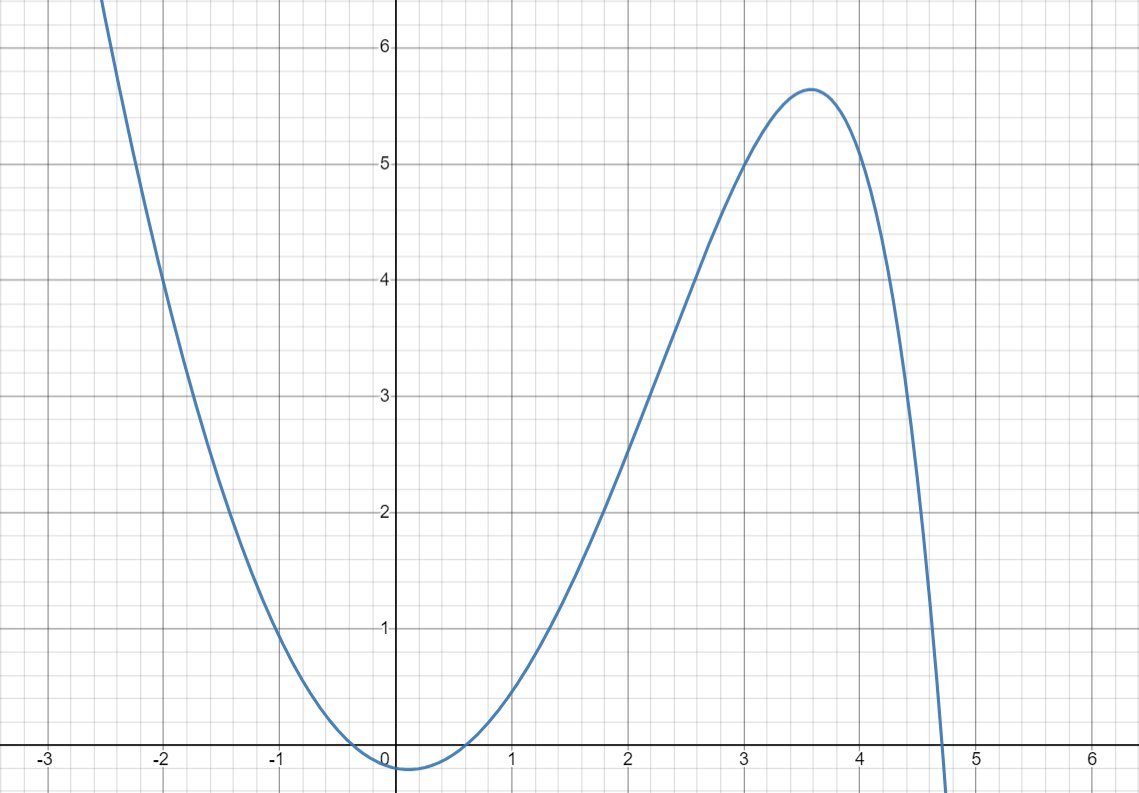
\includegraphics[width=\linewidth]{Pictures/x2_ex_5}
			\caption{График функции $f(x) = x^2 - e^x / 5$}
			\label{x2}
		\end{figure}
		
		У этого уравнения 3 корня. Оценим области их локализации:
		\begin{itemize}
			\item $x_1 \in [-1, 0]$
			
			\item $x_2 \in [0, 1]$
			
			\item $x_3 \in [4, 5]$
		\end{itemize}
	
		Данной локализации достаточно для нахождения корней численным способом.
		
		Теперь построим методы для отыскания корней. Для каждого участка будет свой метод.
		
		\begin{itemize}
			\item $x_1 \in [-1, 0]$. Для этого построим $x^{n + 1} = -\sqrt{\dfrac{\displaystyle e^{x^n}}{5}}$.
			
			Здесь $\varphi(x) = -\sqrt{\dfrac{\displaystyle e^{x}}{5}}$. 
			
			Производная: $\varphi'(x) = -\dfrac{1}{2\sqrt{5}}e^{x / 2}$.
			
			$|\varphi'(x)| \leqslant |\varphi'(0)| = \dfrac{1}{2\sqrt{5}} < 1$. Поэтому данный метод сходится при любом начальном приближении на $[-1, 0]$. Возьмем $x^0 = -1$.
			\\
			
			\item $x_2 \in [0, 1]$. Тут построим почти аналогичный метод: $x^{n + 1} = \sqrt{\dfrac{\displaystyle e^{x^n}}{5}}$.
			
			Здесь $\varphi(x) = \sqrt{\dfrac{\displaystyle e^{x}}{5}}$. 
			
			Производная: $\varphi'(x) = \dfrac{1}{2\sqrt{5}}e^{x / 2}$.
			
			$|\varphi'(x)| \leqslant |\varphi'(1)| = \dfrac{\sqrt{e}}{2\sqrt{5}} < 1$. Поэтому данный метод сходится при любом начальном приближении на $[0, 1]$. Возьмем $x^0 = 0$.
			\\ 
			
			\item $x_3 \in [4, 5]$. Здесь уже чуть-чуть посложнее, но тоже ничего особенного: $x^{n + 1} = \ln(5(x^n)^2)$.
			
			Здесь $\varphi(x) = \ln(5x^2)$. 
			
			Производная: $\varphi'(x) = \dfrac{2}{x}$.
			
			$|\varphi'(x)| \leqslant \varphi'(4) = 0.5 < 1$. Поэтому данный метод сходится при любом начальном приближении на $[4, 5]$. Возьмем $x^0 = 4$.
		\end{itemize}
	
		В качестве невязки берем $r = |f(x_{\text{sol}})| = |x_\text{sol}^2 - e^{x_\text{sol}} / 5|$.
		
		
		\newpage
		\tocsubsection{Результаты}
		При заданном количестве итераций $N = 200$ получаем такие результаты:
		\begin{itemize}
			\item $x_1 = -0.3714177524591739$ с невязкой $r = 0.0$. Очевидно, что она не является нулем. Просто компьютерной точности недостаточно, чтобы посчитать столь малое число. Поэтому считаем $r < \varepsilon^f$ -- точность чисел с плавающей точкой на конкретной машине. 
			
			
			\item $x_2 =  0.6052671213146185$ с невязкой $r = 5.551115123125783 \cdot 10^{-17}$
			
			\item $x_3 =  4.7079379181288585$ с невязкой $r = 7.105427357601002 \cdot 10^{-15}$
		\end{itemize}
	
		При заданной точности $\varepsilon = 1 \cdot 10^{-10}$ имеем следующее:
		\begin{itemize}
			\item $x_1 = -0.3714177524911431$ с невязкой $r = 2.815803146205553 \cdot 10^{-11}$ и 14 итерациями
			
			\item $x_2 = \;\;\, 0.6052671212468322$ с невязкой $r = 5.722416984710321 \cdot 10^{-11}$ и 19 итерациями
			
			\item $x_3 = \;\;\, 4.7079379181231298$ с невязкой $r = 7.304024052245950 \cdot 10^{-11}$ и 30 итерациями
		\end{itemize}
		
		
		Как видим, оба способа сходятся к одному и тому же. Найденные корни также соответствуют \hyperref[x2]{\textcolor{blue}{графику}}.
		
		
		
		\newpage
		\tocsection{Нелинейные системы}
		\tocsubsection{Постановка задачи}
		
		В качестве нелинейных систем были выбраны два пункта: \textbf{IV.12.5 а)} и \textbf{IV.12.7 а)} соответственно:
		\begin{equation*}
			\begin{cases}
				\sin(x + 1) - y = 1.2,\\
				2x + \cos y = 2;
			\end{cases}
			\hspace{30mm}
			\begin{cases}
				2x^2 - xy - 5x + 1 = 0,\\
				x + 3\lg x - y^2 = 0.
			\end{cases}
		\end{equation*}
	
		\tocsubsection{Первая система}
		По порядку разберемся с этими системами. Сначала первая.
		\begin{equation*}
			\begin{cases}
				\sin(x + 1) - y - 1.2 = 0,\\
				2x + \cos y - 2 = 0.
			\end{cases}
		\end{equation*}
		
		\begin{figure}[h!]
			\centering
			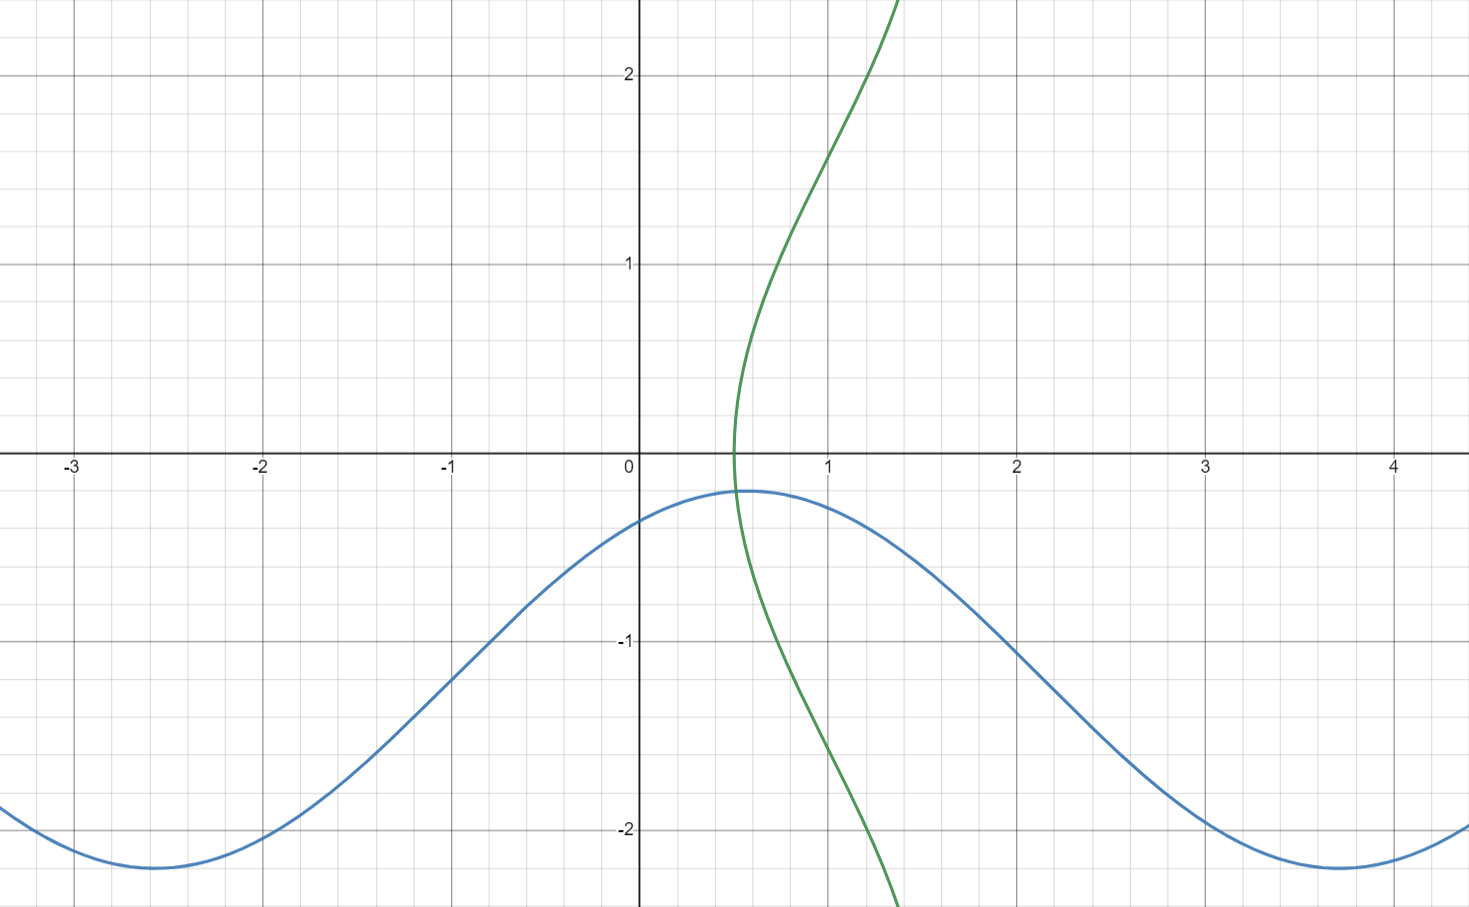
\includegraphics[width=\linewidth]{Pictures/System1}
			\caption{Графики уравнений системы: синим -- ее первое уравнение, зеленым -- второе}
			\label{System1}
		\end{figure}
	
		У нее всего 1 решение, локализованное на $[0.4, 0.6]\times[-0.3, -0.1]$.
		
		Используем метод Ньютона. Для начала посчитаем матрицу Якоби:
		\begin{equation*}
			J = \begin{pmatrix}
				\displaystyle\frac{\partial f_1}{\partial x} & \displaystyle\frac{\partial f_1}{\partial y}\\
				\displaystyle\frac{\partial f_2}{\partial x} & \displaystyle\frac{\partial f_2}{\partial y}
			\end{pmatrix} = 
			\begin{pmatrix}
				\cos(x + 1) & -1 \\
				2 & -\sin y
 			\end{pmatrix}
		\end{equation*}
	
		Непосредственно сам метод Ньютона:
		\begin{equation*}
			\begin{pmatrix}
				x \\
				y
			\end{pmatrix}_{n+1} = 
			\begin{pmatrix}
				x \\
				y
			\end{pmatrix}_{n} - J^{-1}\left[\begin{pmatrix}
				x \\
				y
			\end{pmatrix}_{n}\right] \cdot \vec{F}\left[\begin{pmatrix}
				x \\
				y
			\end{pmatrix}_{n}\right].
		\end{equation*}
	
		Начальным приближением берем $(x, y) = (0.4, -0.3)$.
		В качестве невязки берем $r = \|\vec{F}(\vec{x}_\text{sol})\|_{1, 2, 3}$.
		
		\tocsubsection{Результаты по первой системе}
		При заданном количестве итераций $N = 20$:
		\begin{equation*}
			\begin{pmatrix}
				x \\
				y
			\end{pmatrix} = 
			\begin{pmatrix}
				\;\;\, 0.5101501574507401 \\
				-0.2018384153565740
			\end{pmatrix}
		\end{equation*}
	
		Невязки в разных нормах:
		\begin{itemize}
			\item $r = \|\vec{F}(\vec{x}_\text{sol})\|_{1} < \varepsilon^f$
			
			\item $r = \|\vec{F}(\vec{x}_\text{sol})\|_{2} < \varepsilon^f$
						
			\item $r = \|\vec{F}(\vec{x}_\text{sol})\|_{3} < \varepsilon^f$
		\end{itemize}
		
		Как видим, невязки невероятно малы, даже при 20 итерациях метода! \hyperref[System1]{\textcolor{blue}{График}} подтверждает правильность нахождения решения.
		
		Если же мы попробуем применить метода Ньютона с заданной начальной точностью $\varepsilon = 1 \cdot 10^{-10}$, то получим следующее:
		\begin{equation*}
			\begin{pmatrix}
				x \\
				y
			\end{pmatrix} = 
			\begin{pmatrix}
				\;\;\, 0.5101501574430156 \\
				-0.2018384153268059
			\end{pmatrix},
		\end{equation*}
		\noindent с невязкой $r = 3.97175625721502 \cdot 10^{-11}$ в соответствующей норме. И это всего за $N = 3$ итерации! Сногсшибательная скорость.
		
		
		\newpage
		\tocsubsection{Вторая система}
		Теперь обсчитаем вторую систему.
		\begin{equation*}
			\begin{cases}
				2x^2 - xy - 5x + 1 = 0,\\
				x + 3\lg x - y^2 = 0.
			\end{cases}
		\end{equation*}
	
		\begin{figure}[h!]
			\centering
			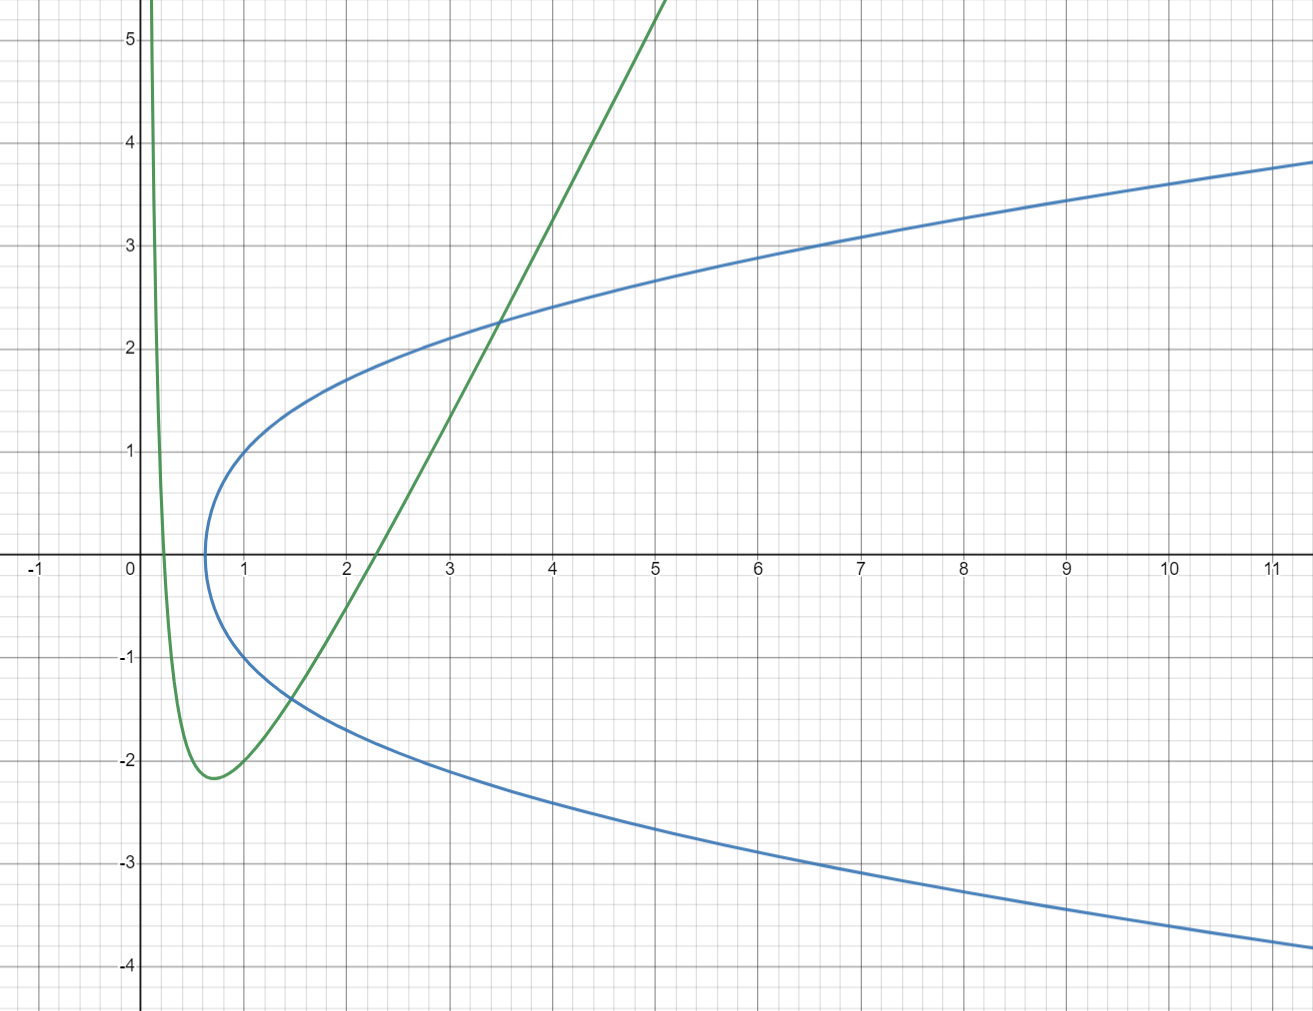
\includegraphics[width=\linewidth]{Pictures/System2}
			\caption{Графики уравнений системы: зеленым -- ее первое уравнение, синим -- второе}
			\label{System2}
		\end{figure}
		У данной системы две точки-решения. Локализуем их:
		\begin{itemize}
			\item $(x_1, y_1) \in [1.4, 1.5] \times [-1.5, -1.3]$
			\item $(x_2, y_2) \in [3.4, 3.5] \times [2.2, 2.3]$
		\end{itemize}
	
		Посчитаем матрицу Якоби:
		\begin{equation*}
			J = \begin{pmatrix}
				\displaystyle\frac{\partial f_1}{\partial x} & \displaystyle\frac{\partial f_1}{\partial y}\\
				\displaystyle\frac{\partial f_2}{\partial x} & \displaystyle\frac{\partial f_2}{\partial y}
			\end{pmatrix} = 
			\begin{pmatrix}
				4x - y - 5 & -x \\
				1 + \dfrac{3}{x \ln 10} & -2y
			\end{pmatrix}.
		\end{equation*}
	
		Для нахождения первой точки-решения возьмем начальное приближение $(x, y) = (1.4, -1.5)$, а для второй --- $(x, y) = (3.5, 2.3)$.
	
		
		\tocsubsection{Результаты по второй системе}
		Для первой точки получаем следующее. При заданном количестве $N = 20$ итераций:
		\begin{equation*}
			\begin{pmatrix}
				x_1 \\
				y_1
			\end{pmatrix} = 
			\begin{pmatrix}
				\;\;\, 1.4588902301521778 \\
				-1.3967670091816180
			\end{pmatrix}
		\end{equation*}
	
		Невязки в разных нормах:
		\begin{itemize}
			\item $r = \|\vec{F}(\vec{x}_\text{sol})\|_{1} < \varepsilon^f$
			
			\item $r = \|\vec{F}(\vec{x}_\text{sol})\|_{2} < \varepsilon^f$
			
			\item $r = \|\vec{F}(\vec{x}_\text{sol})\|_{3} < \varepsilon^f$
		\end{itemize}
	
		При заданной начальной точности $\varepsilon = 1 \cdot 10^{-10}$:
		\begin{equation*}
			\begin{pmatrix}
				x_1 \\
				y_1
			\end{pmatrix} = 
			\begin{pmatrix}
				\;\;\, 1.4588902301513955 \\
				-1.3967670091833093
			\end{pmatrix}
		\end{equation*}
		\noindent с невязкой $r = 6.926903495241277 \cdot 10^{-12}$ за $N = 3$ итерации.
		
		Для второй точки при заданном количестве $N = 20$ итераций:
		\begin{equation*}
			\begin{pmatrix}
				x_1 \\
				y_1
			\end{pmatrix} = 
			\begin{pmatrix}
				\;\;\, 3.4874427876429537 \\
				2.2616286305535938
			\end{pmatrix}
		\end{equation*}
		
		Невязки в разных нормах:
		\begin{itemize}
			\item $r = \|\vec{F}(\vec{x}_\text{sol})\|_{1} = 8.881784197001252 \cdot 10^{-16}$
			
			\item $r = \|\vec{F}(\vec{x}_\text{sol})\|_{2} = 8.881784197001252 \cdot 10^{-16}$
			
			\item $r = \|\vec{F}(\vec{x}_\text{sol})\|_{3} = 8.881784197001252 \cdot 10^{-16}$
		\end{itemize}
		
		При заданной начальной точности $\varepsilon = 1 \cdot 10^{-10}$:
		\begin{equation*}
			\begin{pmatrix}
				x_1 \\
				y_1
			\end{pmatrix} = 
			\begin{pmatrix}
				\;\;\, 3.4874427876429537 \\
				2.2616286305535942
			\end{pmatrix}
		\end{equation*}
		\noindent с невязкой $r = 8.881784197001252 \cdot 10^{-16}$ за $N = 3$ итерации.
		
		По \hyperref[System2]{\textcolor{blue}{графику}} видно, что решения верны.
		
		\newpage
		\tocsection{Вывод}
		В данной работе мы реализовали методы решения нелинейных уравнений и нелинейных систем. Пронаблюдали их достоинства и недостатки. Метод простой итерации требует конкретики задачи и области локализации, поскольку он может медленно сходиться или вовсе не сходиться. Метод Ньютона в этом смысле более универсальный, при этом имеет существенно большую скорость сходимости. Однако он требует бóльших вычислительных затрат. В общем и целом, решения данных нам уравнений и систем были найдены быстро и безболезненно, причем с достаточной точностью.
	
\end{document}